\documentclass[twocolumn]{article}
\usepackage[pdftex]{graphicx}


\title{Lab 1: Simple Harmonic Motion}
\author{Jason Soo}

\begin{document}
\maketitle
\section{Introduction} % (fold)
\label{sec:introduction}
Simple harmonic motion is the motion of a simple harmonic oscillator, a motion that is neither driven nor damped. The motion is periodic, as it repeats itself at standard intervals in a specific manner - described as being sinusoidal, with constant amplitude. It is characterized by its amplitude (which is always positive), its period which is the time for a single oscillation, its frequency which is the number of cycles per unit time, and its phase, which determines the starting point on the sine wave. The period, and its inverse the frequency, are constants determined by the overall system, while the amplitude and phase are determined by the initial conditions (position and velocity) of that system.

Simple harmonic motion is defined by the differential equation
\begin{equation}
	m\frac{d^2x}{dt^2} = -kx
\end{equation}
where ``k'' is a positive constant, ``m'' is the mass of the body, and ``x'' is its displacement from the mean position.

In words, simple harmonic motion is ``motion where the force acting on a body and thereby acceleration of the body is proportional to, and opposite in direction to the displacement from its equilibrium position'' (i.e. $F = -kx$).

A general equation describing simple harmonic motion is 
\begin{equation}
	x(t) = Acos(2\pi ft + \phi)
\end{equation}

where x is the displacement, A is the amplitude of oscillation, $f$ is the frequency, $t$ is the elapsed time, and $\phi$ is the phase of oscillation. If there is no displacement at time $t = 0$, the phase 

\begin{equation}
	\phi = \frac{\pi}{2}
\end{equation}

A motion with frequency $f$ has period

\begin{equation}
	T = \frac{1}{f}
\end{equation}

Simple harmonic motion can serve as a mathematical model of a variety of motions and provides the basis of the characterization of more complicated motions through the techniques of Fourier analysis.
% section introduction (end)

\section{Theory} % (fold)
\label{sec:theory}
When an object exhibits periodic motion (something that can be attributed to a trig function of some sort), the object is said to be in \textbf{harmonic motion}. The most easily understood and fundamental type of this is known as Simple Harmonic Motion (SHM).\\
\\
A string that is stretched past its point of equilibrium and allowed to contract freely will exhibit SHM. If observed, it's very easy to see a spring in such motion is periodic, and excluding all external forces, it would continue to move this way perpetually.\\
\\
A pendulum will operate in the same fashion. When pulled to one side and allowed to fall, the pendulum will oscillate between it's point of equilibrium, showing a constant gain/loss of potential/kinetic energy. If done in a vacuum, it would continue like this forever.
% section theory (end)


\section{Equipment List} % (fold)
\label{sec:equipment_list}
\begin{itemize}
\item[*] Ring Stand
\item[*] Spring
\item[*] Masses
\item[*] Timer
\item[*] Function Generator
\item[*] DC Power Source
\item[*] Oscilloscope
\end{itemize}
% section equipment_list (end)



\section{Procedure}\label{sec:procedure}
\subsection{Part A}\label{sub:part_a}
We attached the spring to a ring stand and hung a mass from the end of the spring. Holding the mass at the springs equilibrium point, we let it drop and the spring was allowed to oscillate. The time for 10 oscillations was recorded. This was repeated several times to get an average time, and was repeated five times for different masses.

\subsection{Part B}\label{sub:part_b}
We attached a string to the ring stand and hung a mass from the other end. The mass was displaced to one side and allowed to swing freely. Once again, we recorded the time for 10 oscillations. This was repeated several times to get an average time, and was repeated five times with different lengths of string.

\subsection{Part C}\label{sub:part_c}
We set the generator to a specific frequency of known value, and measurements were taken. This was done multiple times, and the measurements were then used to compare the given frequency to the frequency read by the oscilloscope.

\section{Data} % (fold)
\label{sec:data}

\subsection{Part A} % (fold)
\label{sub:part_a}

Vertical Spring Motion Results

	\begin{tabular}{cccc}
	\textbf{Mass} & \textbf{Time} & \textbf{T} & \textbf{$T^2$}\\
	\hline
	80g & 8.2s & .82s & .6724s\\
	\hline
	100g & 9.1s & .91s & .8281s\\
	\hline
	120g & 10.0s & 1s & 1s\\
	\hline
	140g & 10.6s & 1.06s & 1.1236s\\
	\hline
	160g & 11.3s & 1.13s & 1.2769s\\
	\hline
	\end{tabular}
	% subsection part_a (end)
	
	\subsection{Part B} % (fold)
	\label{sub:part_b}
		
	Simple Pendulum Results
	
	\begin{tabular}{cccc}
	\textbf{Length} & \textbf{Time} & \textbf{T} & \textbf{$T^2$}\\
	\hline
	100cm & 19.8s & 1.98s & 3.9204s\\
	\hline
	88cm & 18.6s & 1.86s & 3.4596s\\
	\hline
	78cm & 17.3s & 1.73s & 2.9929s\\
	\hline
	65cm & 15.8s & 1.58s & 2.4964s\\
	\hline
	52cm & 14.2s & 1.42s & 2.0164s\\
	\end{tabular}
	
	% subsection part_b (end)

% section data (end)


\section{Analysis of Data}\label{sec:analysis_of_data}

\subsection{Part A}\label{sub:part_a}
The equation we used to relate the mass and the spring to the time it takes to complete an oscillation is
\begin{equation}
	T = 2 \pi \sqrt{\frac{m}{k}}
\end{equation}
By squaring both sides of the equation, we get
\begin{equation}
	T^2 = \frac{4 \pi^2}{k} m
\end{equation}
When the time is squared, and the mass attached to the spring are plotted in a linear fashion, the slope of the line is equal to $\frac{4 \pi^2}{k}$. The value of $k$ can then be found by using the equation
\begin{equation}
	k = -\frac{mg}{x}
\end{equation}
\\
\\
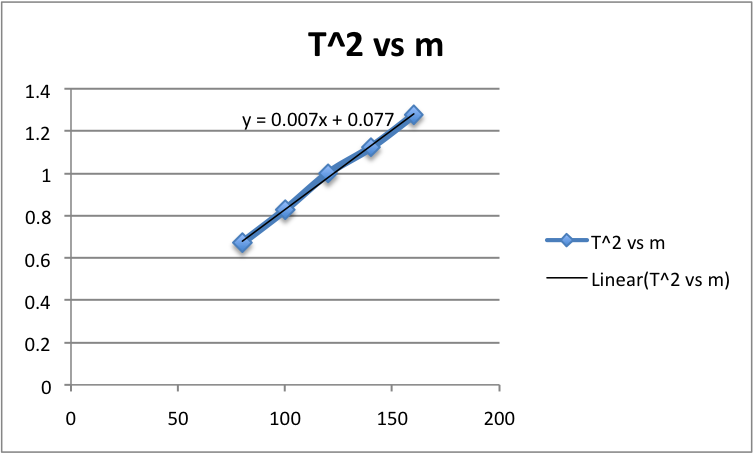
\includegraphics[scale=0.65]{t2vsm.png}
\\
Using the approximate slope we have calculated, we can derive the constant $k$.

\[
	0.007 = \frac{4 \pi^2}{k}
\]
\[
	k = 5639.77
\]


\subsection{Part B}\label{sub:part_b}
The three main factors of this experiment, the gravitational acceleration, the period of the oscillation and the length of the string of the pendulum are all related through the equation
\begin{equation}
	T = 2 \pi \frac{L}{g}
\end{equation}
We can do some minor manipulation to the equation and get a more useful one
\begin{equation}
	T^2 = \frac{4 \pi^2}{g} L
\end{equation}
When this function is plotted, it yields a linear regression, with the slope of the line being represented by $\frac{4 \pi^2}{g}$.
\\
\\
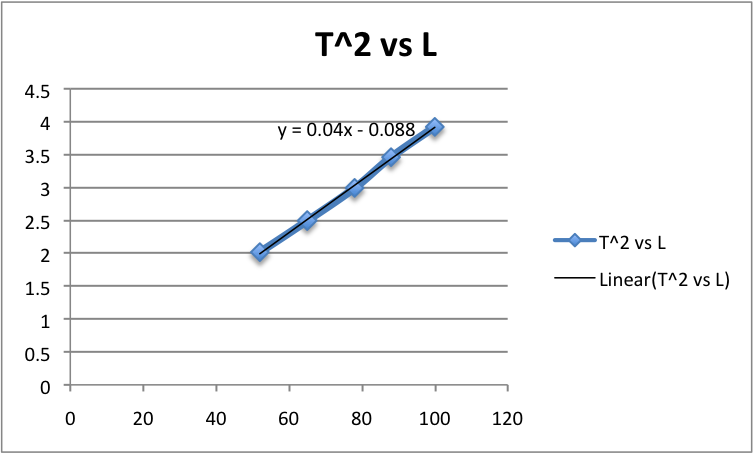
\includegraphics[scale=.65]{t2vsl.png}
\\
Now that we have an approximate regression line, we can use this to determine the value of $g$

\[
	.04 = \frac{4 \pi^2}{g}
\]
\[
	g = 9.869 \frac{m}{s^2}
\]


\section{Conclusions}\label{sec:conclusions}
The relatively accurate and consistent results provided by our data reinforces the validity of the equations presented to us in class. You can see this by looking at the tables for Part A and B. It is very clear that the linear regression is quite accurate based on our data, and the linear regression calculates the constants $k$ and $g$ accurately.

\end{document}